\documentclass{beamer}
\usecolortheme{wolverine}

% math stuff
\usepackage{amsmath}
\usepackage{amsthm}
\usepackage{amssymb}
\usepackage{xcolor}

\usepackage{float}
\usepackage{subcaption}

% to insert images
\usepackage{graphicx}

% to correctly insert stressed characters
\usepackage[T1]{fontenc}
\usepackage[utf8]{inputenc}

\usepackage{multirow}

% Bibliography
% \usepackage[style=alphabetic]{biblatex}
% \usepackage[nottoc]{tocbibind}
% \usepackage{bibentry}
% \setcounter{biburllcpenalty}{9000}
% \usepackage{nameref}

% to put links in table of contents
\usepackage{hyperref}
\hypersetup{colorlinks=false, %set true if you want colored links
    linktoc=all,     %set to all if you
}

% Add symbols
% \usepackage{textcomp}

% Add command for Real and Z sets
% \usepackage{dsfont}
% \newcommand{\Rset}{$\mathds{R}$}
% \newcommand{\Zset}{$\mathds{Z}$}

% Code highlighting
% \usepackage{minted}
% \usemintedstyle{perldoc}
% \setminted{
%     frame=single,
%     breaklines,
% }

% tikz figures
% \usepackage{tikz}
% \input{style.tikzstyle}
% \usetikzlibrary{positioning}

% number rounding
\usepackage{siunitx}
\sisetup{round-mode=places,round-precision=5}

\definecolor{myyellow}{RGB}{225, 225, 0}

\begin{document}
\title{Thesis notes}
\date{9th March}
\frame{\titlepage}

\begin{frame}[c]
    \frametitle{A graph on @nytimes (1)}
    \begin{figure}[htpb]
        \centering
        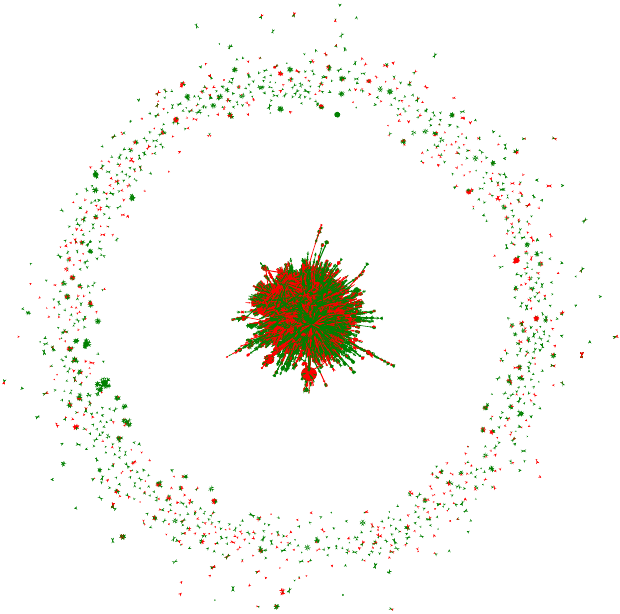
\includegraphics[width=0.8\linewidth]{img/nytimes.png}
        % \caption{out/nytimes400/Graph}%
        % \label{fig:out/nytimes400/graph}
    \end{figure}
\end{frame}

\begin{frame}[c]
    \frametitle{A graph on @nytimes (2)}
    \begin{itemize}
        \item The graph has 42161 vertices and 74505 edges
        \item Fraction of negative edges: \num{0.504476209650359}
        \item Clustering coefficient: \num{0.00029194931947211565} with
            standard deviation \num{0.0011972202917824519}
        \item Average shortest path length: \num{12.386406147989614}
        \item Median shortest path length: \num{12.0}
        \item Average degree: \num{3.5343089585161644}
        \item Unique average degree: \num{2.313322739024217}
    \end{itemize}
\end{frame}

% Thread lowest negative edge fraction top 3:
%     https://twitter.com/user/status/1367890148369731586 with 0.0
%     https://twitter.com/user/status/1367203191750811649 with 0.0
%     https://twitter.com/user/status/1367610889726283785 with 0.0
% Thread highest negative edge fraction top 3:
%     https://twitter.com/user/status/1367047646385483777 with 1.0
%     https://twitter.com/user/status/1367444681336889349 with 1.0
%     https://twitter.com/user/status/1367175821757136899 with 1.0
% Content lowest negative edge fraction top 3:
%     https://www.nytimes.com/2021/03/03/technology/personaltech/peloton-alternatives-at-home-workout.html with 0.0
%     https://www.nytimes.com/2021/03/04/business/ministry-of-supply-pandemic-clothing.html with 0.0
%     https://www.nytimes.com/2021/03/04/travel/finding-refuge-and-a-snowy-owl-in-central-park.html with 0.0
% Content highest negative edge fraction top 3:
%     https://www.nytimes.com/2021/03/03/us/wisconsin-wolves-killings.html with 0.6794751640112465
%     https://www.nytimes.com/2021/03/03/world/asia/myanmar-protests-violence.html with 0.6633266533066132
%     https://www.nytimes.com/2021/03/04/us/politics/merrick-garland-justice-department.html with 0.6521739130434783

\begin{frame}[c]
    \frametitle{A graph on @nytimes (3)}
    \begin{figure}[htpb]
        \centering
        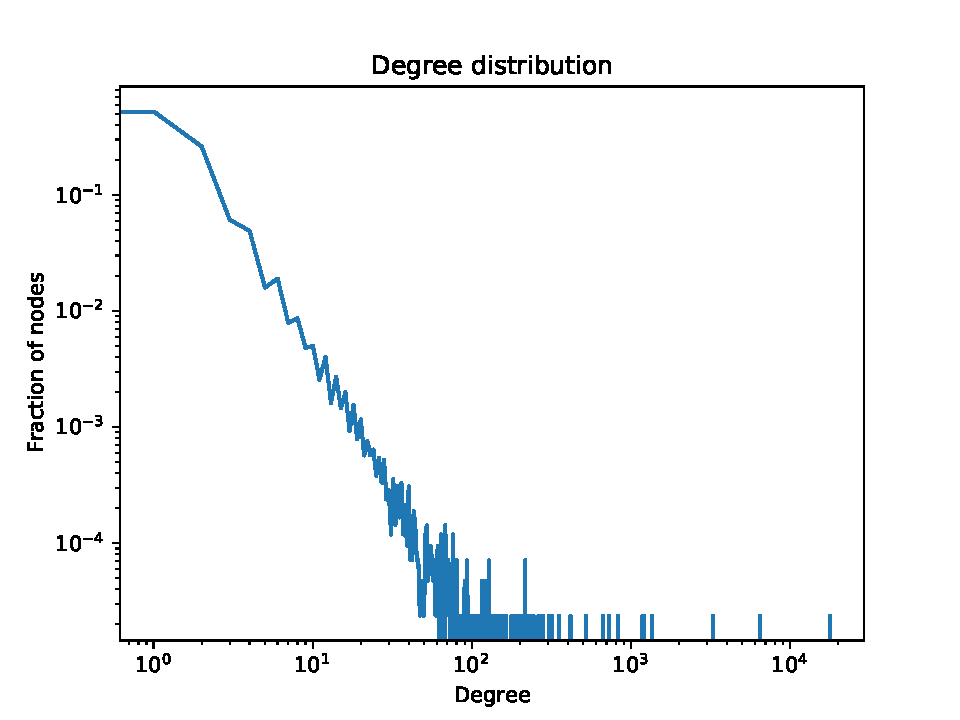
\includegraphics[width=0.8\linewidth]{out/nytimes400/degree-dist.pdf}
        % \caption{out/nytimes400/degree-Dist}%
        % \label{fig:out/nytimes400/degree-dist}
    \end{figure}
\end{frame}



\begin{frame}[c]
    \frametitle{A graph on @nytimes (4)}
    \begin{figure}[htpb]
        \centering
        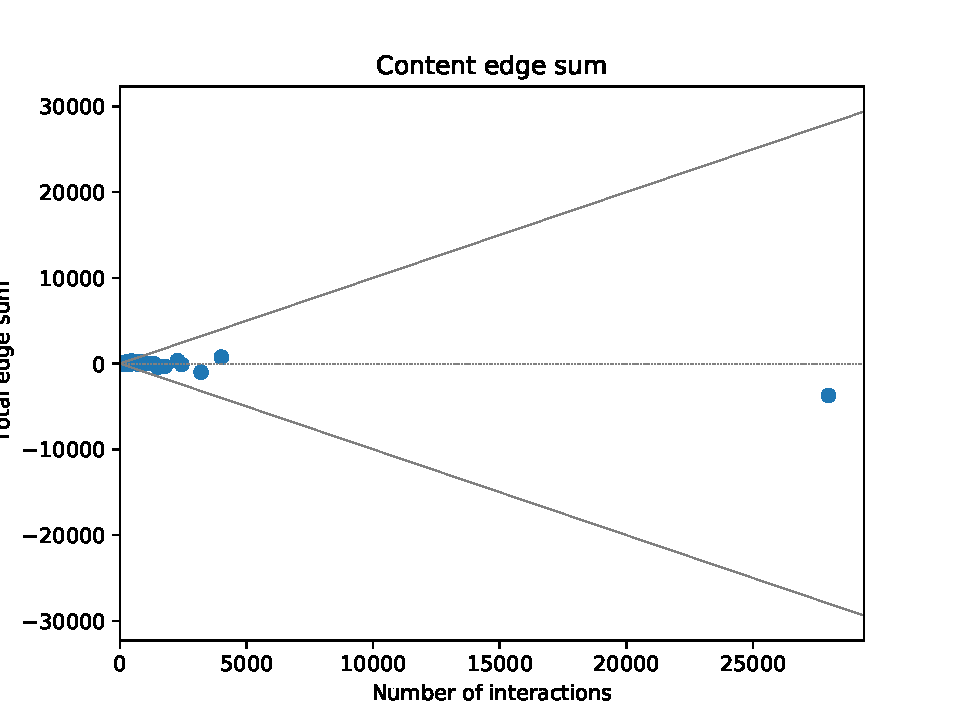
\includegraphics[width=0.8\linewidth]{out/nytimes400/edge-sum-n-interactions.pdf}
        % \caption{out/nytimes400/edge-sum-n-Interactions}%
        % \label{fig:out/nytimes400/edge-sum-n-interactions}
    \end{figure}
\end{frame}

\begin{frame}[c]
    \frametitle{A graph on @nytimes (4)}
    \begin{figure}[htpb]
        \centering
        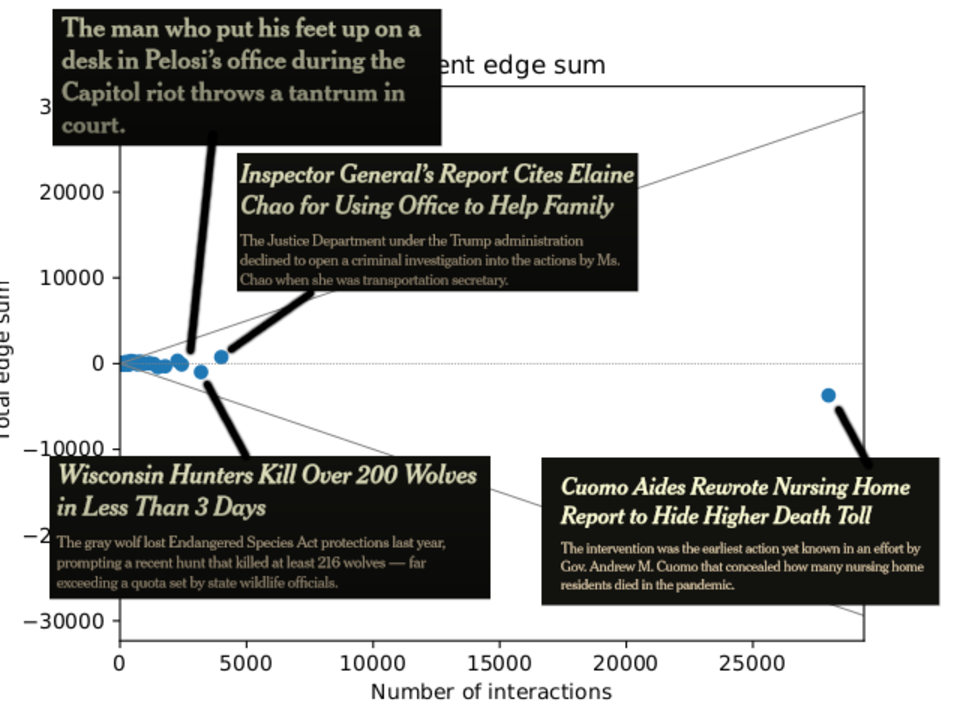
\includegraphics[width=0.8\linewidth]{img/edge-sum-n-interactions-labeled.pdf}
        % \caption{img/edge-sum-n-interactions-Labeled}%
        % \label{fig:img/edge-sum-n-interactions-labeled}
    \end{figure}
\end{frame}

\begin{frame}[c]
    \frametitle{A graph on @nytimes (5)}

    Least discussed contents:

    \begin{figure}[htpb]
        \centering
        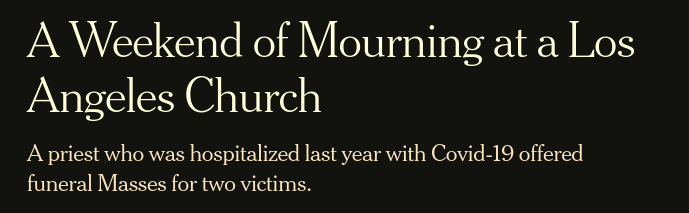
\includegraphics[width=0.5\linewidth]{img/ndiscussed1.png}
        % \caption{img/Ndiscussed1}%
        % \label{fig:img/ndiscussed1}
    \end{figure}

    \begin{figure}[htpb]
        \centering
        
\includegraphics[width=0.5\linewidth]{img/ndiscussed2.png}
        % \caption{img/Ndiscussed2}%
        % \label{fig:img/ndiscussed2}
    \end{figure}

    \begin{figure}[htpb]
        \centering
        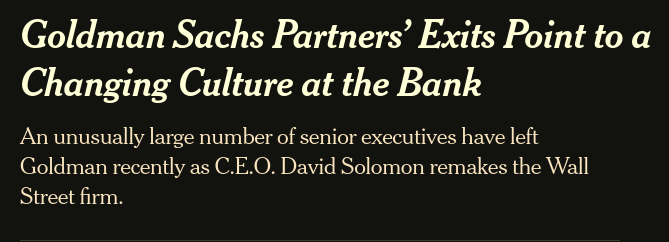
\includegraphics[width=0.5\linewidth]{img/ndiscussed3.png}
        % \caption{img/Ndiscussed3}%
        % \label{fig:img/ndiscussed3}
    \end{figure}

\end{frame}

\begin{frame}[c]
    \frametitle{A graph on @nytimes (6)}
    \begin{figure}[htpb]
        \centering
        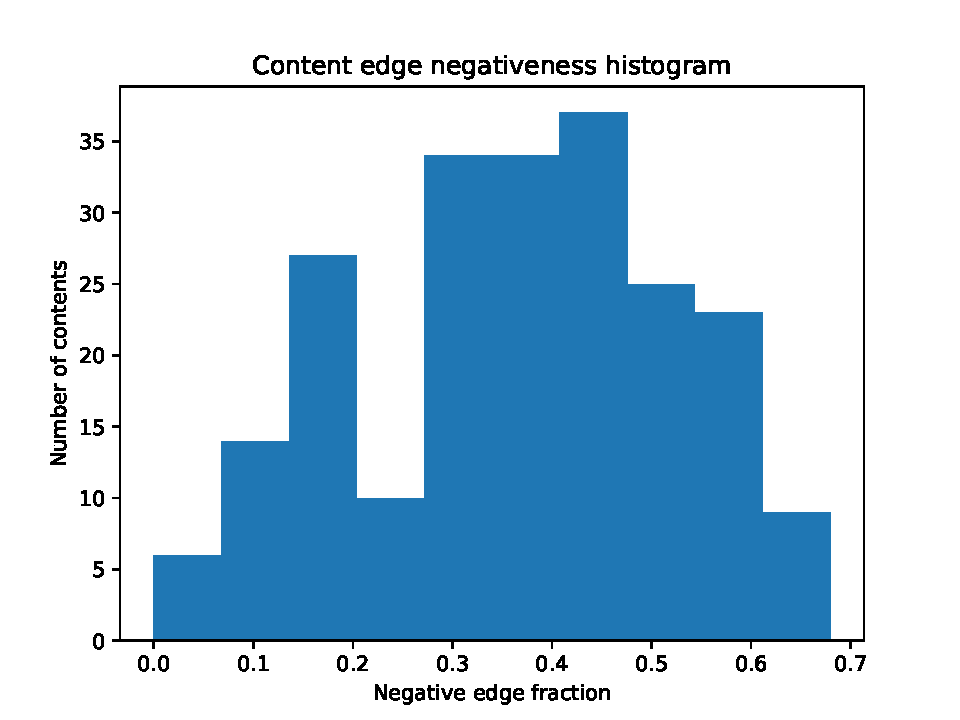
\includegraphics[width=0.8\linewidth]{out/nytimes400/neg-fraction-content-hist.pdf}
        % \caption{out/nytimes400/neg-fraction-content-Hist}%
        % \label{fig:out/nytimes400/neg-fraction-content-hist}
    \end{figure}
\end{frame}


\begin{frame}[c]
    \frametitle{A graph on @nytimes (7)}

    \begin{figure}[htpb]
        \centering
        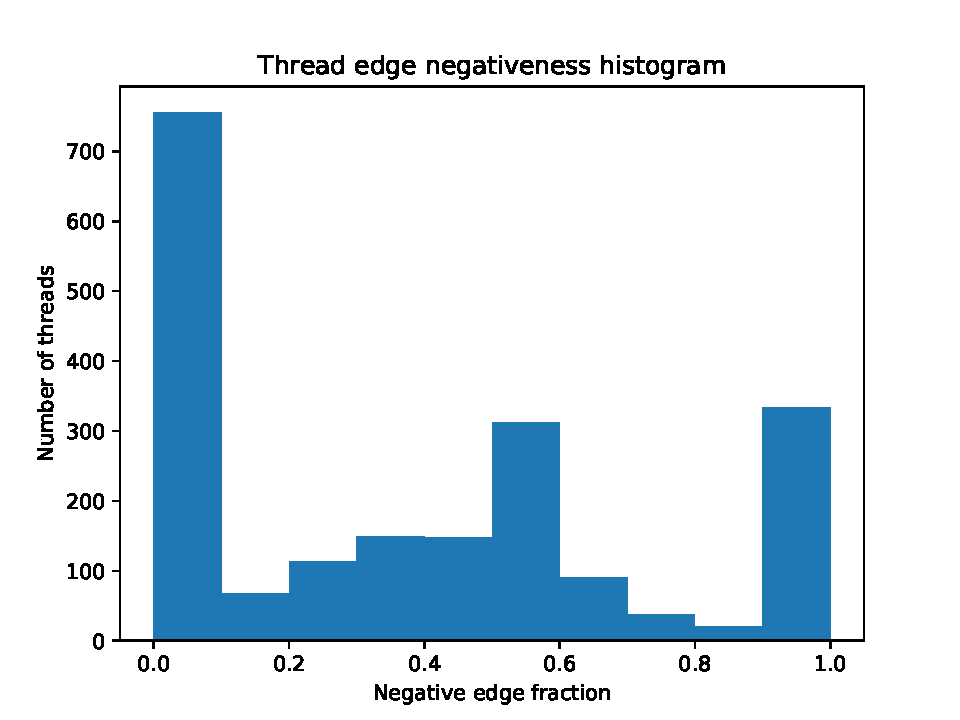
\includegraphics[width=0.8\linewidth]{out/nytimes400/neg-fraction-thread-hist.pdf}
        % \caption{out/nytimes400/neg-fraction-thread-Hist}%
        % \label{fig:out/nytimes400/neg-fraction-thread-hist}
    \end{figure}
\end{frame}

\begin{frame}[c]
    \frametitle{A graph on @nytimes (8)}

    \begin{figure}[htpb]
        \centering
        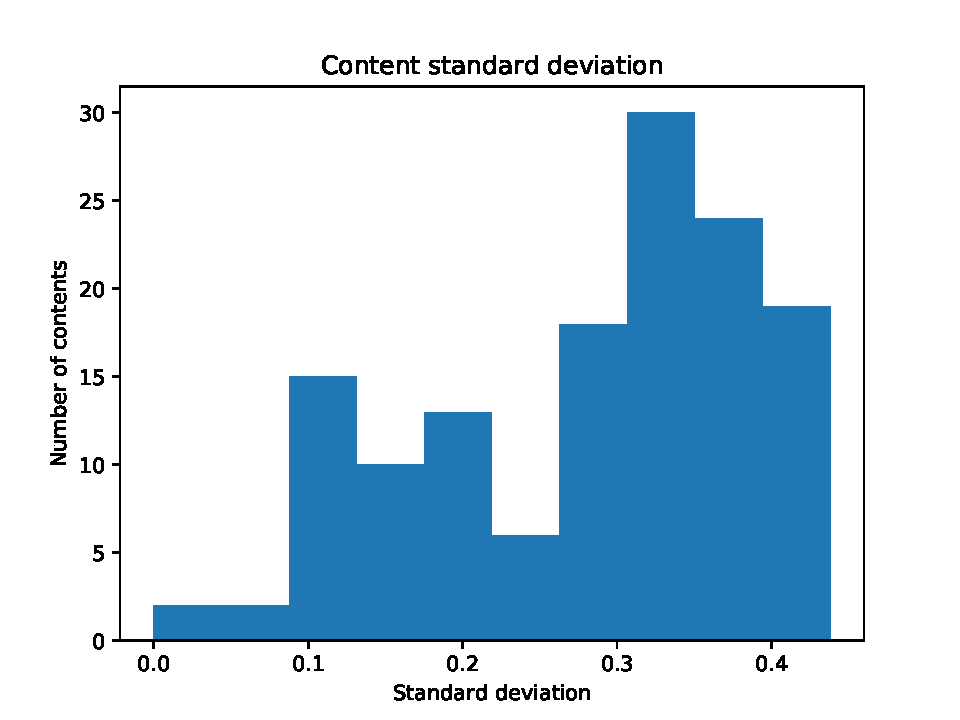
\includegraphics[width=0.8\linewidth]{out/nytimes400/content-std-dev-hist.pdf}
        % \caption{out/nytimes400/content-std-dev-Hist}%
        % \label{fig:out/nytimes400/content-std-dev-hist}
    \end{figure}
\end{frame}

\begin{frame}[c]
    \frametitle{Contents with low standard deviation}
    \begin{figure}[htpb]
        \centering
        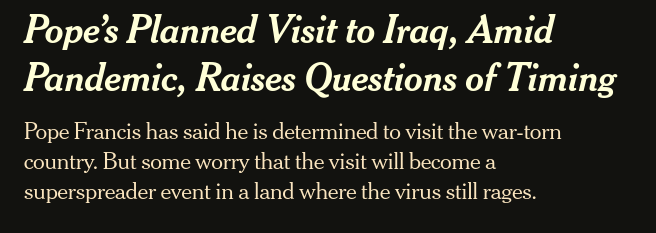
\includegraphics[width=0.5\linewidth]{img/low_stddev/1.png}
        % \caption{img/low_stddev/1}%
        % \label{fig:img/low_stddev/1}
    \end{figure}

    \begin{figure}[htpb]
        \centering
        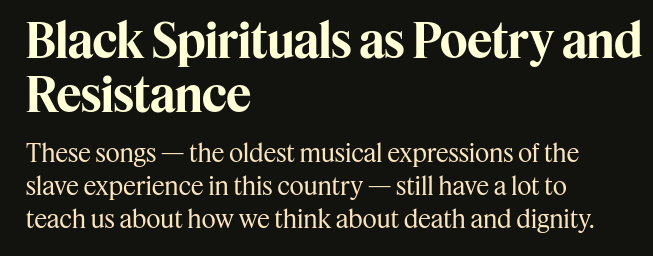
\includegraphics[width=0.5\linewidth]{img/low_stddev/2.png}
        % \caption{img/low_stddev/1}%
        % \label{fig:img/low_stddev/1}
    \end{figure}
    \begin{figure}[htpb]
        \centering
        
\includegraphics[width=0.5\linewidth]{img/low_stddev/3.png}
        % \caption{img/low_stddev/1}%
        % \label{fig:img/low_stddev/1}
    \end{figure}
\end{frame}


\begin{frame}[c]
    \frametitle{Contents with high standard deviation}
    \begin{figure}[htpb]
        \centering
        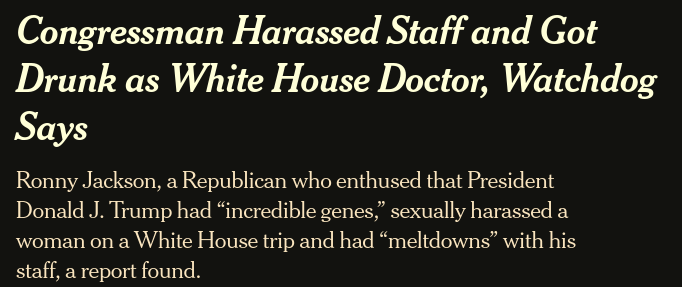
\includegraphics[width=0.5\linewidth]{img/high_stddev/1.png}
        % \caption{img/high_stddev/1}%
        % \label{fig:img/high_stddev/1}
    \end{figure}

    \begin{figure}[htpb]
        \centering
        
\includegraphics[width=0.5\linewidth]{img/high_stddev/2.png}
        % \caption{img/high_stddev/1}%
        % \label{fig:img/high_stddev/1}
    \end{figure}
    \begin{figure}[htpb]
        \centering
        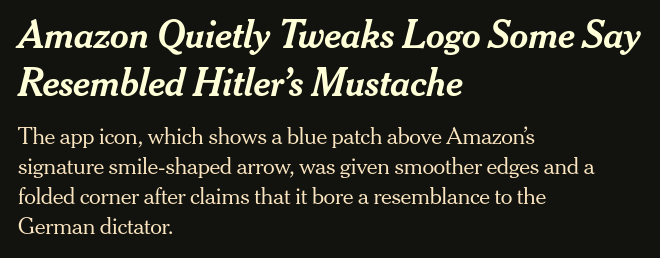
\includegraphics[width=0.5\linewidth]{img/high_stddev/3.png}
        % \caption{img/high_stddev/1}%
        % \label{fig:img/low_stddev/1}
    \end{figure}
\end{frame}

\begin{frame}[c]
    \frametitle{A content-user graph on r/AskTrumpSupporters}
    \begin{figure}[htpb]
        \centering
        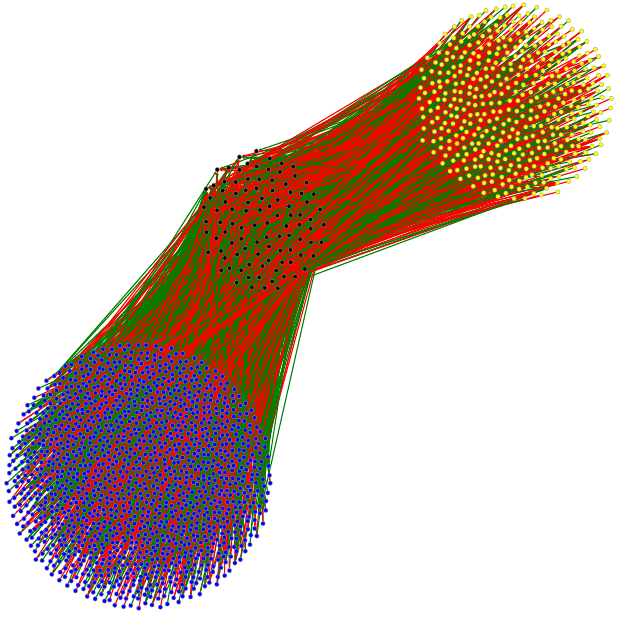
\includegraphics[width=0.8\linewidth]{img/exp-graph.png}
        % \caption{img/exp-Graph}%
        % \label{fig:img/exp-graph}
    \end{figure}
\end{frame}

\begin{frame}[c]
    \frametitle{A content-user graph on r/AskTrumpSupporters}
    \begin{figure}[htpb]
        \centering
        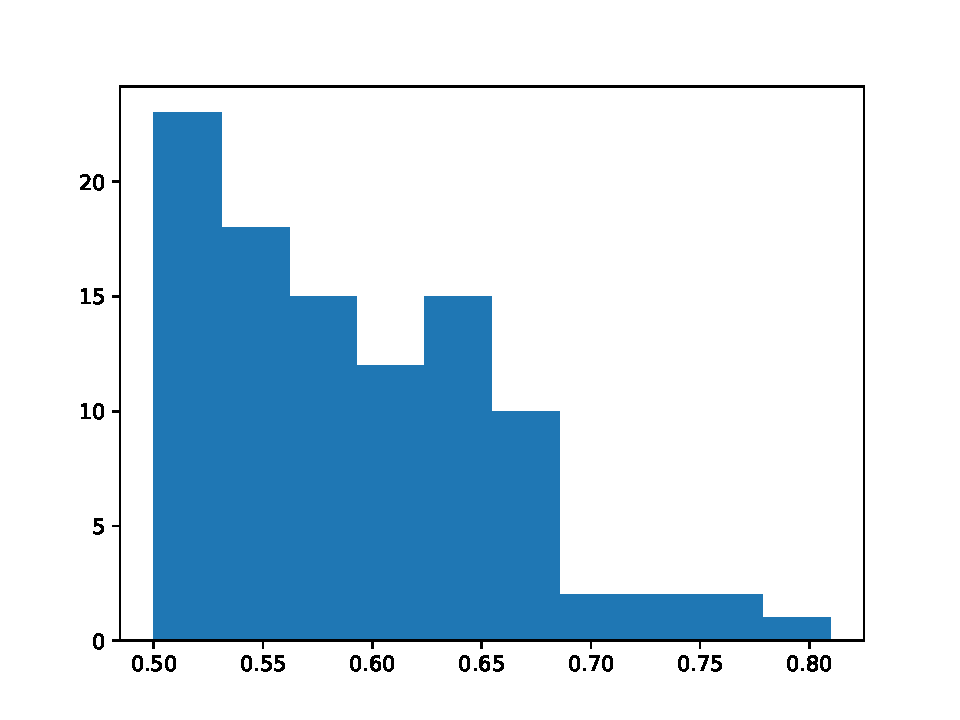
\includegraphics[width=0.8\linewidth]{out/experimental200/experimental200-accuracy-hist.pdf}
        \caption{Content accuracy in classifying users}%
        \label{fig:out/experimental200/experimental200-accuracy-hist}
    \end{figure}
\end{frame}

\begin{frame}[c]
    \frametitle{A content-user graph on r/AskTrumpSupporters}

    \begin{itemize}
        \item \textit{Were there some legitimate scandals during the Trump presidency?
                If so, what were they and how do you think they will rank among
            other presidential scandals in history?} (0.80)
            {\tiny
            \url{https://www.reddit.com/r/AskTrumpSupporters/comments/l0qos6/were_there_some_legitimate_scandals_during_the/}}
        \item \textit{What are your thoughts on the Democrat Voting bill being
            introduced (again) to Congress?} (0.77)
            {\tiny
            \url{https://www.reddit.com/r/AskTrumpSupporters/comments/lve318/what_are_your_thoughts_on_the_democrat_voting/}}
        \item \textit{Weekend} (off-politics post) (0.75)
            {\tiny\url{https://www.reddit.com/r/AskTrumpSupporters/comments/lo5fcf/weekend/}}
        \item  \textit{Why are you a partisan?} (0.72)
            {\tiny\url{https://www.reddit.com/r/AskTrumpSupporters/comments/l0e943/why_are_you_a_partisan/}}
    \end{itemize}

\end{frame}

\end{document}


